% Verificare utilizzo della parola "tutorial" per eventualmente rimuoverla. Lo scopo del libroo è avere un manuale completo, non solo un tutorial.

\part{Getting started}

\chapter{Starting a new project}
After the installation of Tomb Editor pack, you are ready to make your very first Tomb Engine project. (Level map file extensions are well-known as “PRJ” files, but do not misunderstand: what we call “project” now is not a level, but a whole level set - i.e. your current Tomb Engine game itself, which will be released when you fully made it.)
\par But where do you need to place your projects? Well, NOT in Tomb Editor main folder - that is a place you usually never modify while editing. I suggest placing all of your projects nicely collected in a so-called general project folder. This could be called eg. \path{"My_Tomb_Raider_projects"}, created manually. (I created it in Documents folder.)
\par Each project you make will be placed in its own main folder. Does it mean now you should also create manually a project main folder in the general folder? No, there is a TombIDE wizard which will do the whole project-creating procedure for you.
\par Projects are handled in \textbf{TombIDE (Tomb Integrated Development Environment or TIDE)} program, that is why the whole project-creating procedure is also being done there.
So start \path{TombIDE.exe}, and the panel of TIDE Start page opens up.
Click on “Create a new project” button now.
The first page of a new panel opens up (General Information, \ref{fig:tide1}):
\begin{figure}
    \centering
     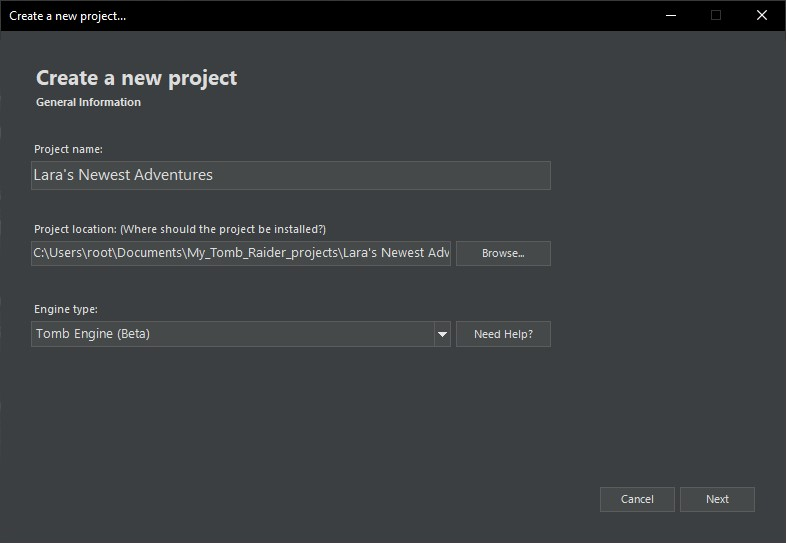
\includegraphics[width=0.75\textwidth]{screenshots/1.jpg}
     \caption{General Information}
     \label{fig:tide1}
\end{figure}

\begin{itemize}
    \item Let's suppose the project you start now has the name of “Lara's Newest Adventures”. So type it now here.
    \item Click on “Browse” button, find and select the general project folder.
    \item After that, the little window in the middle of this first page shows that a subfolder in the general project folder will be created as the main folder of this project, having the project name.
    \item The engine type you choose now is naturally Tomb Engine.
\end{itemize}


\par Now click on “Next” button to continue the procedure on the next page of the panel (Extra Options, \ref{fig:tide2}).

\begin{figure}
    \centering
     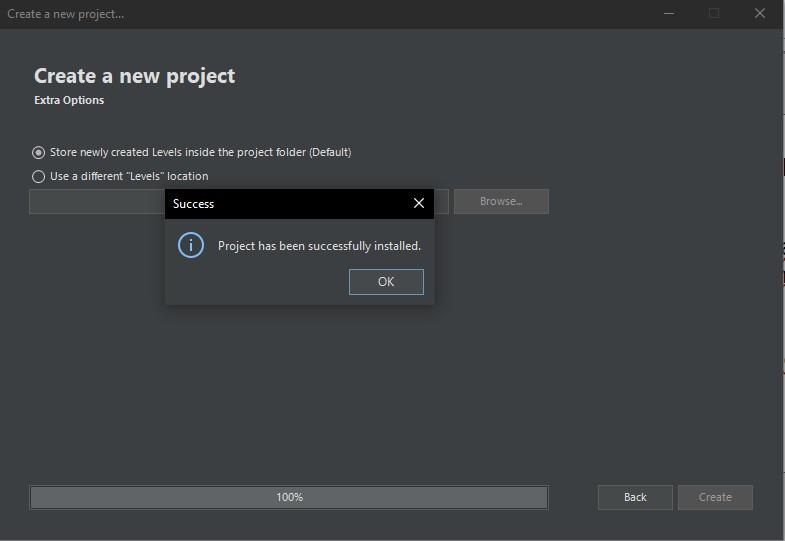
\includegraphics[width=0.75\textwidth]{screenshots/2.jpg}
     \caption{Extra Options}
     \label{fig:tide2}
\end{figure}

\par I suggest changing nothing here. Which means level map files will be handled in a folder called "Levels", which is a subfolder in the main folder of the project. (I mean, this is the default place for level map files, and you, the beginner probably should keep it like this.)
\par Now click on "Create" button here, then look at the increasing bar at the bottom of the panel.
When the bar is at 100 \%, then you get a message that the project has been successfully created (\ref{fig:tide3}).

\begin{figure}
    \centering
     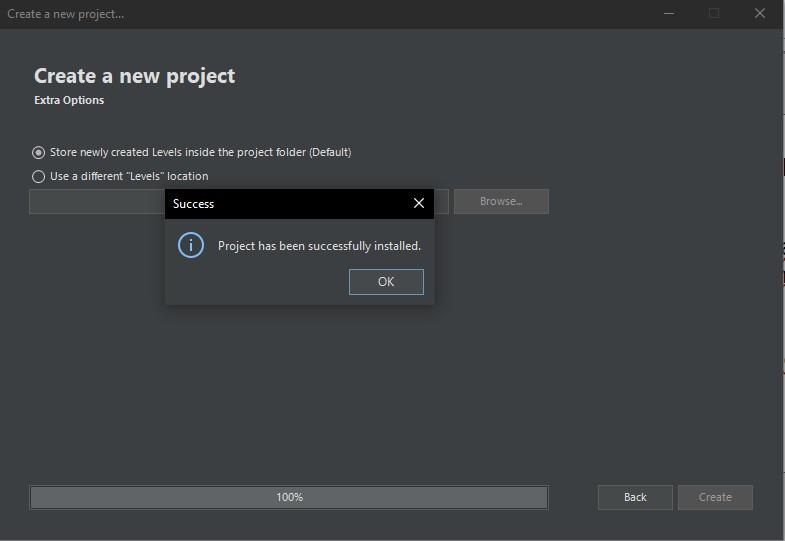
\includegraphics[width=0.75\textwidth]{screenshots/3.jpg}
     \caption{Project has been successfully installed}
     \label{fig:tide3}
\end{figure}

\par And this project main folder has been also created on the selected route, with the basic contents a TEN project should have. (Including Levels folder - still being empty - in that default position., \ref{fig:tide4})

\begin{figure}
    \centering
     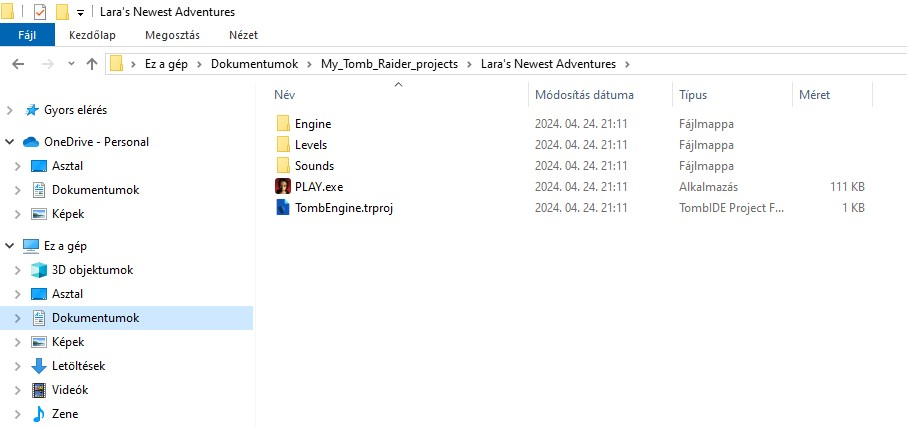
\includegraphics[width=0.75\textwidth]{screenshots/4.jpg}
     \caption{Project directories have been created (Since TEN 1.7., the project main folder has an Assets subfolder as well.)}
     \label{fig:tide4}
\end{figure}

Double-click on that row (or click on "Open selected button" below), so the project opens in TIDE, you will be able to work on it. Each project opened in TIDE has more pages, now you can see its Level Manager page. (See the panel header which names the current project.)
% \par Now click on the red arrow in the upper left corner of the page, to go back to TIDE Start page, closing this project now in TIDE. (Since TEN 1.7., you can see the blue TIDE icon in that corner, instead of the red arrow. If you click on that icon, then a menu opens. One of the menu options is an arrow, with "Back to Start Window..." name. Click on it to go back to TIDE Start page.) \cite{akyv_tutorial} % Referring to old version, changed to fit latest version
\par Now click on the blue TIDE icon in the upper left corner of the page, then a menu opens. One of the menu options is an arrow, with "Back to Start Window..." name. Click on it to close this project now, going back to TIDE Start page.
\cite{akyv_tutorial}

\chapter{What is a level?}
Before we discuss how to start a new level, important to understand, that actually what a "level" is.
\emph{(Don't do anything now, just read and listen.)}
\section{Level map}
Level maps are the editable versions of levels. So when you create, modify a level in the level editor program, then the changes are saved and stored in level map files.
 TE has its own level map formula, whose extension is called \path{PRJ2}.\footnote{Previously level map files was known as files with \path{PRJ} extension.}
 \par At the moment you don't have PRJ2 files, but soon you will create them and save them in Levels folder of the project main folder. (In fact, in subfolders of Levels folder, and each subfolder is dedicated only to one level of the project, having a name which nicely refers to the level name.)
 \section{Playable level}
 The playable version of the level is a level file what the game will play as a level. This playable file is made by a conversion, converted from the PRJ2 level map file of this level. (The conversion will be a very simple task to you: only a simple click on a button.)
 \section{Level script}
Script means game or level data, described simply by typing some texts.
There is a tool in TE pack dedicated to edit script. This is TIDE you have already used to create your project, and you definitely will use it later much to edit your script. \footnote{In TRLE or NGLE there is a "level block" in the script, where all the scripted data of that level are typed. In TE it works the same way - except if the engine for your TE project is TEN. In that case script works a bit differently, as you will see. (Though, a level block also exists there.)}
\section{Item files}
An item file (attached to a level) contains all the Moveable and Static objects (Lara, creatures, statues, furniture, effect emitters etc.) and sprites \footnote{In computer graphics, a \textbf{sprite} is a two-dimensional bitmap that is integrated into a larger scene, most often in a 2D video game. \cite{sprite_wikipedia} \index{Sprite}} which can be used in that level.
In TE you can select more than one item file for a level. (And if an object is there in both, then you can set which one of them should be applied in the level.)
\footnote{Unlike the older editors, where only one item file could be selected per level.}
\begin {itemize}
    \item \par Builders using TRLE/NGLE previously definitely know that the extension of an item file is \path{WAD}, acronym standing for \emph{Where's All the Data?} \footnote{WAD is generally a main architectural component of retro games - see e.g. \url{https://en.wikipedia.org/wiki/Doom_modding} for usage in \emph{Doom} custom games.}, made/edited probably with WadMerger program. But it is not obvious any more, if your level editor program is Tomb Editor. In TE WAD extension is usually supported, but not preferred.
    \item \path{WAD2} extension means an enhanced item file (eg. with the feature of UV-mapping \footnote{\textbf{UV mapping} is the 3D modeling process of projecting a 3D model's surface to a 2D image for texture mapping. The letters "U" and "V" denote the axes of the 2D texture because "X", "Y", and "Z" are already used to denote the axes of the 3D object in model space. \cite{UV_mapping_wikipedia} \index{UV mapping}} which is not possible in WAD files). WAD2 files are made and useable only for TE levels, it is the preferred extension here. \\ There is a tool in TE pack dedicated to edit item files, called WadTool. Just open a WAD in it, and save it. It will be saved automatically as a WAD2 item file. (Or you can naturally arrange even a brand new WAD2 in WadTool.)
    \item TEN engine is able to use only specific WAD2 files, which means WAD extension is not supported for TEN engine. (Except if WAD has only objects having non-TEN specific behaviors, like Statics.) \\ You can find a menu option in WadTool, to convert your other item files into a TEN WAD2. \\ "Specific" means eg. TEN Lara object is optimized for TEN, so a "casual" (non-TEN) Lara would not be animated properly there. (Later we discuss it in this tutorial - but not the details, because it is not a TEN WAD2 tutorial.)
\end{itemize}
WAD2 files for a TEN level should be placed in Levels folder, in the subfolder of that level. (It is recommended to use a sub-subfolder there for it.) - Though, technically it is not a must, they can be placed even anywhere in your computer.
\section{Texture files}
A texture \footnote{A \emph{texture map} \index{Texture map} refers to a 2D image ("texture") that adds visual detail to a 3D model. The image can be stored as a raster graphic. A texture that stores a specific property—such as bumpiness, reflectivity, or transparency—is also referred to as a \emph{color map} or \emph{roughness map}. \cite{texture_mapping_wikipedia}} file (attached to a level) contains all the texture tiles which can be placed on room faces (floor sector, ceiling sector, wall section) in that level.
\par In TE:
\begin{itemize}
    \item you can select more than one texture file for a level, placing tiles even from each in your level,
    \item not only TGA extension is supported for texture files, but even other ones: BMP, JPG, PNG etc.
\end{itemize}
Texture files for a TEN level should be placed in Levels folder, in the subfolder of that level. (It is recommended to use a sub-subfolder there for it.) - Though, technically it is not a must, they can be placed even anywhere in your computer.
\section{Sound files and their catalog files}
Sounds saved in sound files can be emitted mostly by Moveable objects (mostly Lara or other creatures), but even by any effect (like a rumbling earthquake). Etc.
\par Sound files have WAV extensions - just like in the old times.
\par Sound files are not directly attached to a level map, for two reasons:
\begin{itemize}
    \item Sound files for a TEN level should be placed in Sounds subfolder of project main folder. (Though, technically it is not a must, they can be placed even anywhere in your computer.) Initially you can find all the original sounds here of the legacy engines, in their own subfolders. - But naturally you are allowed to edit these contents, modifying, deleting, adding sound files here. \\ These places are needed to be attached to that level.
    \item There must be one catalog file (or, unlike the older editors, even more catalog files), attached to the level, where the sounds you want to attach are named. The main reason is that sounds can have different properties for different levels, and the catalog will describe the properties that this sound will have on this level \\ Sound catalogs can be even older types, familiar from TRLE/NGLE (Sounds.txt or SFX/SAM files of WAD files), or the ones having XML extensions, which are made for TE. Later you will be able to make custom XML files, but some of them are created when saving a WAD2 file. And there are even some preset XML catalogs in Catalogs/TEN Sound Catalogs subfolder of Tomb Editor main folder. \\ There is a tool in TE pack dedicated to edit sound catalogs, called SoundTool. If you want, just open a non-XML catalog into it, and save it as an XML one.
\end{itemize}
\section{Conclusion}
When you start building a new level for your project, then these are your tasks, recommended in this order:
\begin{enumerate}
\item Create a PRJ2 level map file.
\item Add this level to the project.
\item Check the needful contents of the level script. If your script has less contents than that, then the level is useless in the game.
\item Check the main settings (in TE) for the level. If they are wrong, then the level is useless in the game.
\item Check the crucial attachments.
\item You can try to edit something in the level map - then save it.
\item Convert the PRJ2 level map into a TEN playable level.
\item Start the level in the game, try what you have just edited in the map.
\end{enumerate} \cite{akyv_tutorial}

\chapter{Starting a new level map}

\begin{enumerate}
    \item Open the "Lara Newest Adventures" project in TIDE, remaining on Level Manager page.
    \item See the left big window here, with the title of "Level list". As the text says in it, click on it, or - because the text is not available when there is at least one level in this window - click on the "+" button on the upper left corner of the window.
    \item The panel of "Create a New Level" opens (\ref{fig:tide7}):
    \begin{itemize}
        \item \textbf{Level Name}: this level name will be shown in the game for this level. Let's say it is "Test Level 1" now.
        \item \textbf{Use custom PRJ2 / DATA name}: if you tick it, then you can add an alternative name key instead of the default one. \\ Name keys are the names of the most important files of this level. The default name key is mostly the Level Name, except: there cannot be spaces. So eg. for Test Level 1, level files will be auto-created with this name key later: Test\_Level\_1.prj2, Test\_Level\_1.ten etc. \\ Let's suppose we don't want the default name key now, so tick the option and type "Test1" as the name key. (So the file names will be Test1.prj2, Test1.ten etc.)
        \item \textbf{Generate Lua script}: as I said above, there is a scripted part even for TEN. If you untick it, then the wizard will skip this part, not creating the needful contents of the level script. So later you have to create it manually (but before starting the level at the very first time in the game).
        % \\ (The option name is a bit misleading, though, Script.txt and [Level] section are presented in a bit different way for TEN. But it doesn't matter.)%
        \\ Some values in the scripted part you need to define now:
\begin{itemize}
    \item \textbf{Ambient sound ID}: the initial ambient background noise of the level. I suggest accepting this 110.wav now, because later you can change it any time. Or you can click on Open /audio/ button to open Engine \textbackslash Audio subfolder in the project main folder now, to try to find another one. \footnote{Audio subfolder has the original audio file set of The Last Revelation game. Later you can change the contents any time. Now I suggest choosing a WAV above 100 value here, because in that set, background noises are placed on those IDs. However, for TEN you can use any ID for a background noise - but we won't discuss it in this tutorial.}
    \item \textbf{Enable HORIZON (Make the skybox visible in the level)}: the sky above you can be visible in the outdoor areas of the level only if it is ticked. I suggest ticking it, because later you can change it any time. footnote{Skybox and horizon are working together, but they are not the same. But it doesn't matter now.}

\begin{figure}
    \centering
     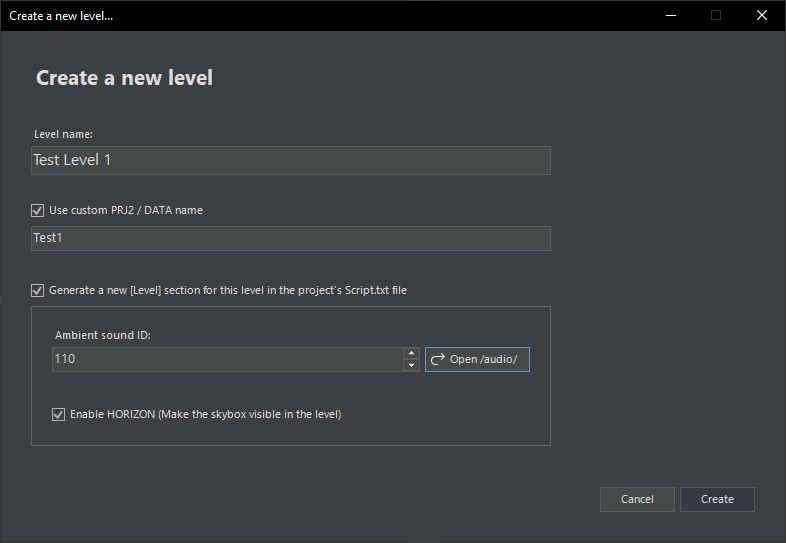
\includegraphics[width=0.75\textwidth]{screenshots/7.jpg}
     \caption{\emph{Create a New Level} panel}
     \label{fig:tide7}
\end{figure}



\end{itemize}
\end{itemize}
\item Click on Create button.
\end{enumerate}

What happened now are:
\begin{itemize}
    \item As I said, each level should have a folder dedicated to it, in Levels folder of this project. Now a dedicated folder to Test Level 1 automatically has been created there, having this level name.
    \item A Test1.prj2 file has been also automatically created, in Test Level 1 folder.
    \item The main settings of this level have also been done properly.
    \item Some crucial attachments of the level has been automatically attached. (Later we discuss it in the tutorial.)
    \item In Level list window of this project (on Level Manager TIDE page), a row for this level has been also automatically created (\ref{fig:tide8}).
    
\begin{figure}
    \centering
     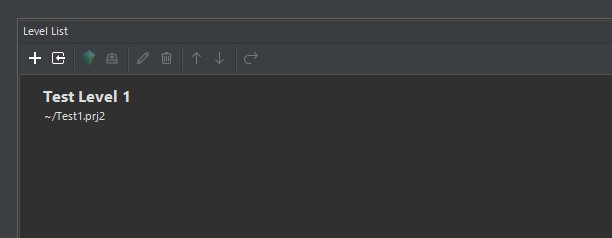
\includegraphics[width=0.75\textwidth]{screenshots/8.jpg}
     \caption{\emph{Level list} panel showing level you've created}
     \label{fig:tide8}
\end{figure}

    \item The needful contents of the level script has been also automatically created. (Later we discuss it in the tutorial.)

\end{itemize}
Now you can click on the arrow menu option in the menu of the blue TIDE icon to go back to the Start page of TIDE.
%\\ But TIDE now asks you if you want to save what you have just did. Naturally accept it. \\ (However, operations you did in TIDE are automatically saved. Except if those are rows typed in the script.) % It was not asked to save by the application during testing of this tutorial...

\chapter{Time to run the first (default) room}

\section{Open your level in \emph{Tomb Editor}}
Once you're in the TombIDE start page, double click on your project \emph{Lara's Newest Adventure} to open it (or alternatively, select the project and click on the "Open selected project" button), then:
\begin{itemize}
    \item double click on your "Test Level 1"
    \item or alternatively, select "Test Level 1", then click on the icon in the upper part of the Level, similar to a green prysm. This is the icon of the \emph{Tomb Editor}.
\end{itemize}
This action will open the Tomb Editor (\ref{fig:te1000}).

\begin{figure}
    \centering
     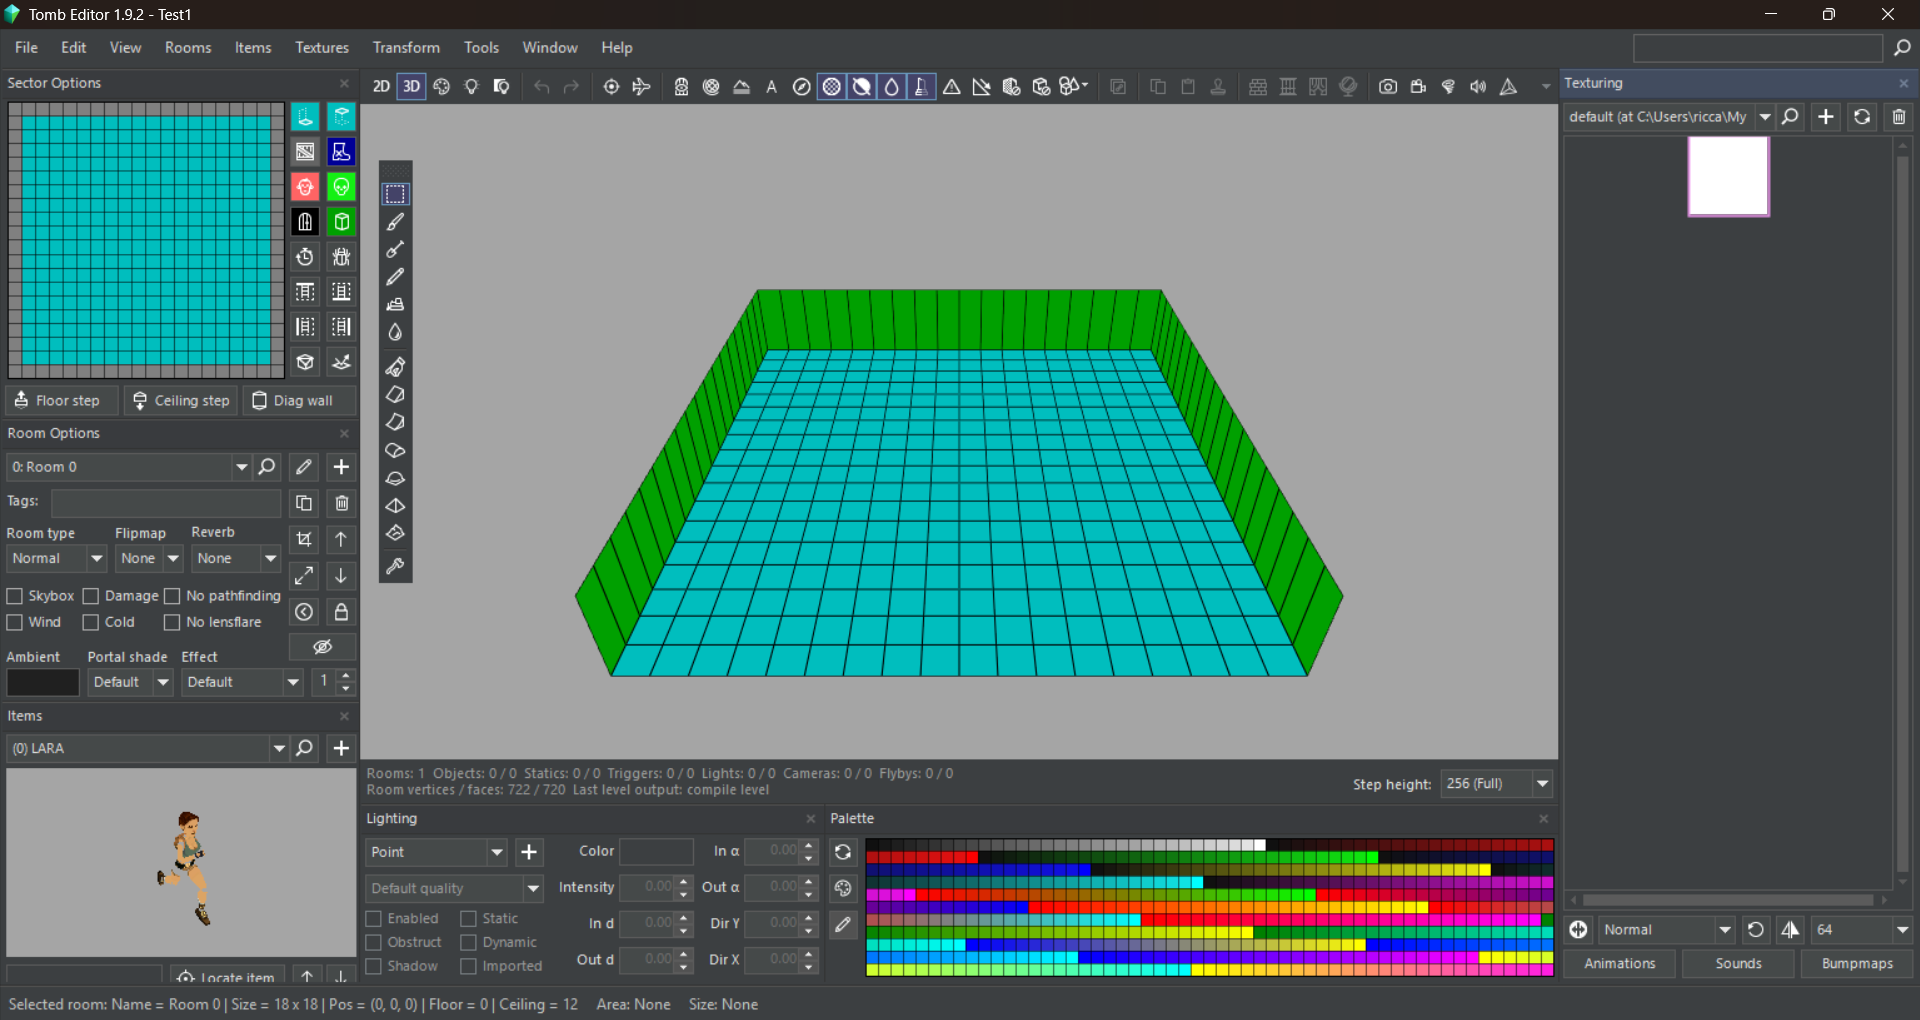
\includegraphics[width=1\textwidth]{screenshots/1000.png}
     \caption{\emph{Tomb Editor} main screen}
     \label{fig:te1000} 
\end{figure}

\section{Default level properties}
When you create a new level, by default the TombIDE tool creates for you a very basic level, containing one squared room, having size 18x18x3.
We'll discuss about size later on in details, talking about blocks, rooms and their properties.
\par For now, just look in front of you: you can see the square room represented in a tridimensional view. You can check this is the 3D view of a rectangular cuboid, by left-clicking on the room and moving the mouse while keeping the left button of the mouse pressed.
\par Please note, this room created by default:
\begin{itemize}
    \item \textbf{is already textured in white} - in other words, basically is fully painted in white color (floor, walls and ceiling).
    \item is dark, since no lights are defined by default. Don't worry about that, we'll plenty discuss about lights later on.
\end{itemize}
Now you're not able to see here this room is white and dark: please, trust me for now.
\par Hey! Do you remember we talked about the \emph{crucial attachments}? Well, when you create a new level, TombIDE automatically adds:
\begin{itemize}
    \item a default \emph{item file}, or WAD, that is a revisited version of objects from TR4
    \item a default \emph{texture file}, containing a single white texture the whole room is automatically "painted" with, as above mentioned
    \item default \emph{sound files and their catalog}, from TR4 as well
\end{itemize}
For now, don't worry about where you can check and change the attachments in Tomb Editor: we'll discuss the through entire chapters dedicated to each of them later on.

\section{Wait! Something is missing...}

There's only one step before we can play the level. Guess what is missing? Our Lara.
\par This is a general rule:
\begin{remark}
A level can be played only if Lara's object is placed into the level.
\end{remark}
To place Lara in the room, it's enough to (\ref{fig:temovelara}):
\begin{itemize}
    \item left click on a floor box inside the room
    \item click on "Move Lara"
\end{itemize}
Now you can see Lara is placed in the room.

\begin{figure}
    \centering
     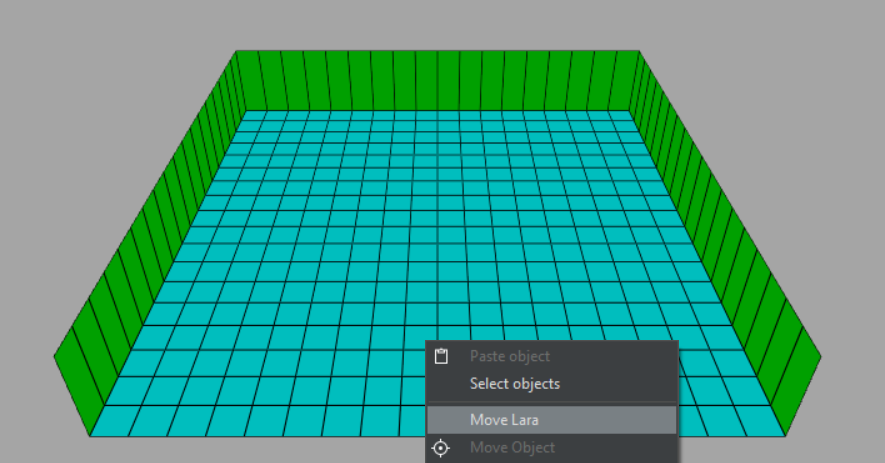
\includegraphics[width=1\textwidth]{screenshots/1001.png}
     \caption{Placing Lara}
     \label{fig:temovelara} 
\end{figure}

\section{Ready to play your first room?}
All done! Now we can build the level and play it by alternatively:
\begin{itemize}
    \item press F5 on the keyboard
    \item or click on the "Build level and play (F5)" button in the top menu.
\end{itemize}
Now the Tomb Engine will build the level for you and run it.
\par Well, I know\dots it's a unique, squared room all painted in white where Lara is trapped forever into: you'll need to close the game manually, cause we've not set anything but Lara's position, neither a way out of the room nor anything to say to the game the level is actually finished. But, \textbf{congratulations}! You've build and run your first level successfully.
\begin{center}
  $\ast$~$\ast$~$\ast$
\end{center}

\par As you've seen, this first level has been actually, fully, automatically generated by the Tomb Integrated Development Environment. In the next chapters, we will see what the application done now for us, having a short overview of the level main settings and components.

\chapter{Overview of \emph{Tomb Editor} UI}

The User Interface of Tomb Editor is composed by different panels or \emph{windows} (\ref{fig:TEUI}):

\begin{enumerate}
    \item \textbf{Editor Window}: main working window for modeling, texturing and viewing in 2D, 3D and preview modes
    \item \textbf{Tool Palette (floating)}
    \item \textbf{Editor Window Buttons}
    \item \textbf{Drop down menu bar}
    \item \textbf{Drop down menu search}: search commands in drop down menu bar by their name
    \item \textbf{Sector Options}: top down view of the selected room; secondary working window
    \item \textbf{Room Options}: create rooms; add/edit features in rooms
    \item \textbf{Item Browser}: preview, select and place objects. Please notice there's Lara here!
    \item \textbf{Lightning}: select, place and adjust lights
    \item \textbf{Palette}: provides colors used for transparency; quick way to assign colors to lights and objects
    \item \textbf{Texture Panel}: select tiles for texturing model; set animation ranges and texture sounds
    \item \textbf{Statistics}: room location and statistics; total number of triggers and objects in project
    \item \textbf{Room info box}
    \item Other windows - \textbf{please note:} by default, the following panels are active in the user interface left bar, but not visible since the bar itself is too short to include them all:
\begin{itemize}
    \item \textbf{Trigger List}
    \item \textbf{Imported Geometry Browser}
\end{itemize}
% Da valutare se segnalare al team di sviluppo. Per me questo è un bug.

\end{enumerate}

\begin{figure}
    \centering
     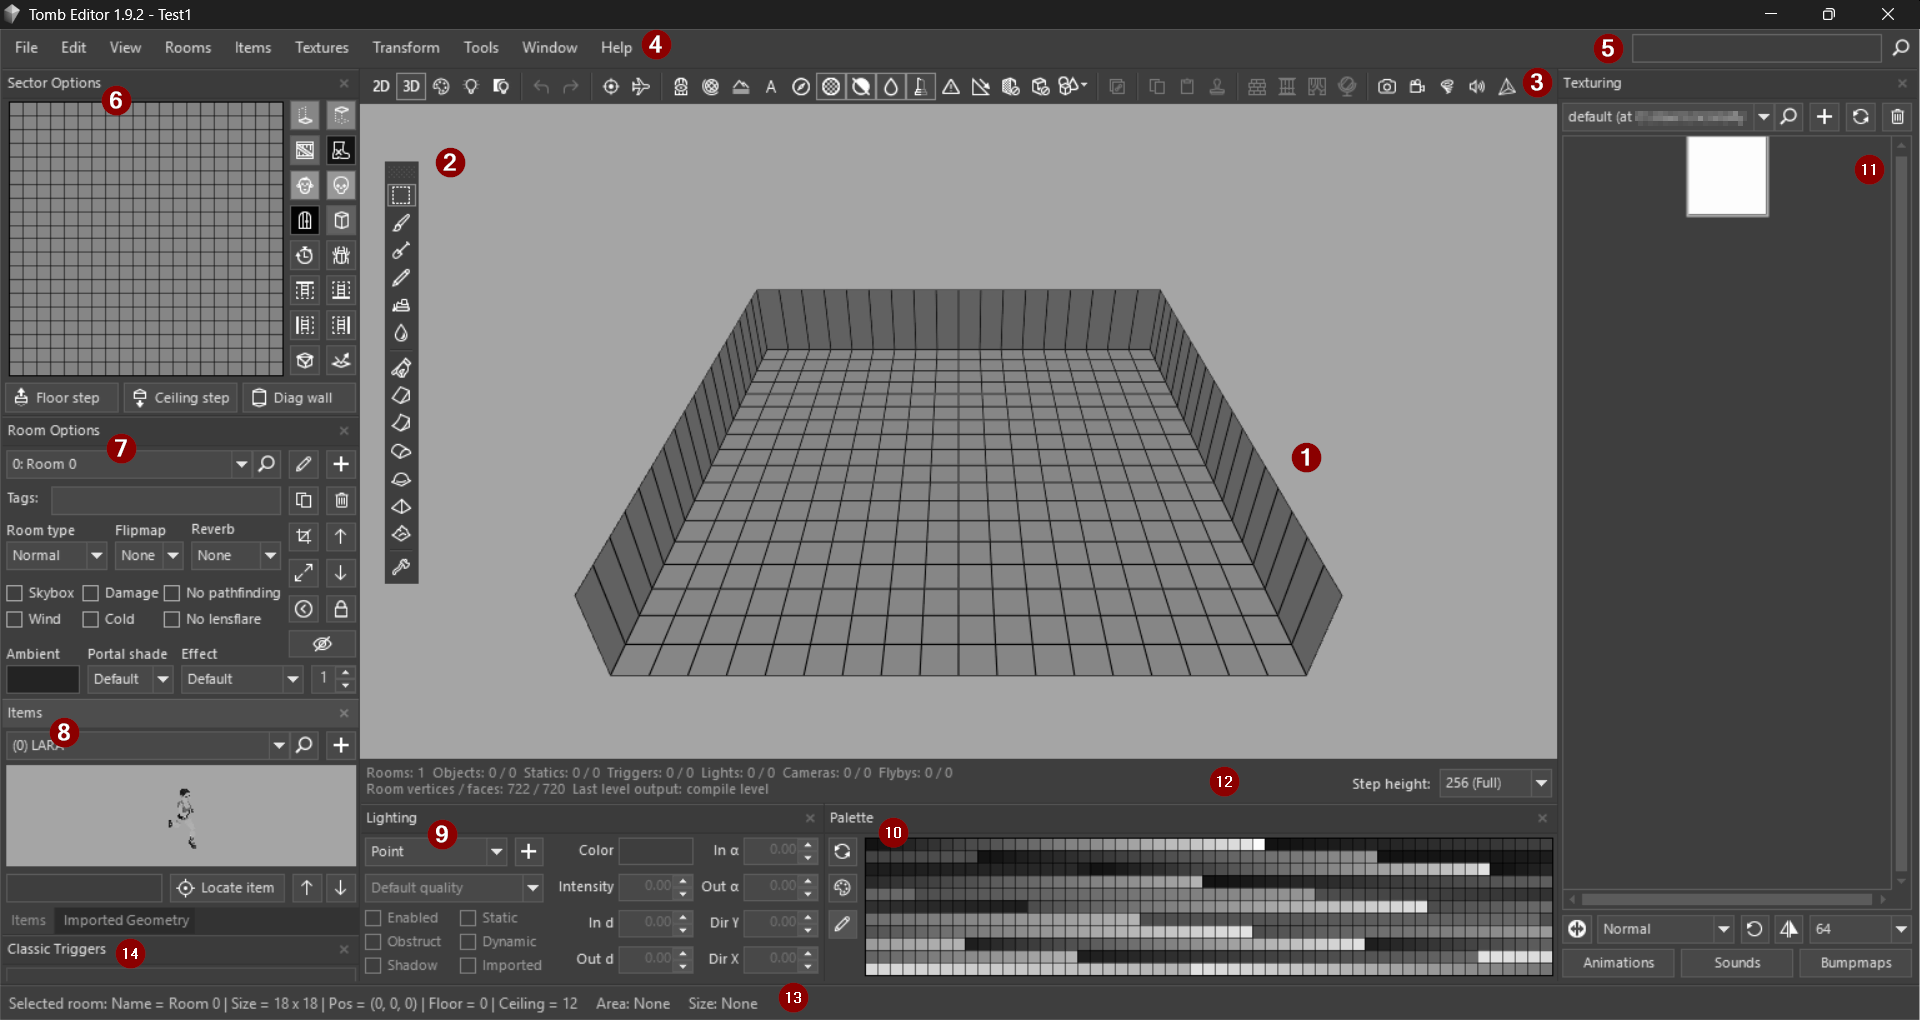
\includegraphics[width=1\textwidth]{screenshots/2025-08-23 17_29_21-Tomb Editor 1.9.2 - Test1.png}
     \caption{Placing Lara}
     \label{fig:TEUI} 
\end{figure}

Panels can be hidden or shown, using the \path{Window} menu bar. As well, here you can restore the default layout.
\par Panels can be moved within the interface, placing them where you prefer by dragging and dropping their title.


\chapter{Main contents of the level scripts}
All the script files for a TEN project are available in \path{Engine \ Scripts} subfolder of the project main folder.
Some of them are not important for us now, and some of them won't be important even later. - So let's see which script files are important, when you start building a new level:
\begin{itemize}
    \item \path{Gameflow.lua}
    \item \path{Strings.lua}
    \item \path{.lua} file with the key level name (in \path{Levels} subfolder of the \path{Scripts} folder), i.e. \path{Test1.lua} now.
\end{itemize}

You can open and edit these script using whatever text editor you'd like. However, there are two integrated ways to open scripts in TombIDE:
\begin{itemize}
    \item Scripting Studio in TombIDE
    \item Visual Studio Code
\end{itemize}

But, first of all: why these files have \path{.lua} extension?

\section{What is Lua?}

\textbf{Lua} is a lightweight and high-level programming language designed mainly for embedded use in applications. Lua is cross-platform software.

\par In video game development, Lua is widely used as a scripting language, mainly due to its perceived ease of embedding, fast execution, and short learning curve. Notable games which use Lua include \emph{Roblox, Garry's Mod, World of Warcraft, Payday 2, Phantasy Star Online 2, Dota 2, Crysis} and many others. Some games that do not natively support Lua programming or scripting have this function added by mod.

\par In 2003, a poll conducted by GameDev.net showed that Lua was the most popular scripting language for game programming. \cite{LUA_Wikipedia}

\par Scripts written in Lua language have \path{.lua} file extension.


\section{Scripting Studio in TIDE}
Once opened the project in TombIDE, you can open the integrated Scripting Studio clicking on the icon \emph{Scripting Studio} on the left. Naturally this is the page where you can edit your script.
\par The main parts of this page are (\ref{fig:TIDEScriptingStudio}):
\begin{itemize}
    \item Dropdown menu.
    \item Toolbar with buttons.
    \item The big window to see/edit the script: any text you can see here is some textual data for your game/level. Or, if a row starts with a \path{--} sign, that means the row is just a comment, a note, so you can type anything here.
    % Verifica se usare path o usare già un ambiente di codice con LUA, sezione immediatamente successiva direi
    \item File Explorer panel on the right side: Here you can find all the available script files of the project.
Click on any file name of File Explorer, to open that file in the big window.
There are tabs above the window, for the script files are just open there. Gameflow.lua are always open initially. (Naturally you can close any tab if you just doesn't care about it any more.) Click on any of those tabs to see its contents in the window.
\end{itemize}

\begin{figure}
    \centering
     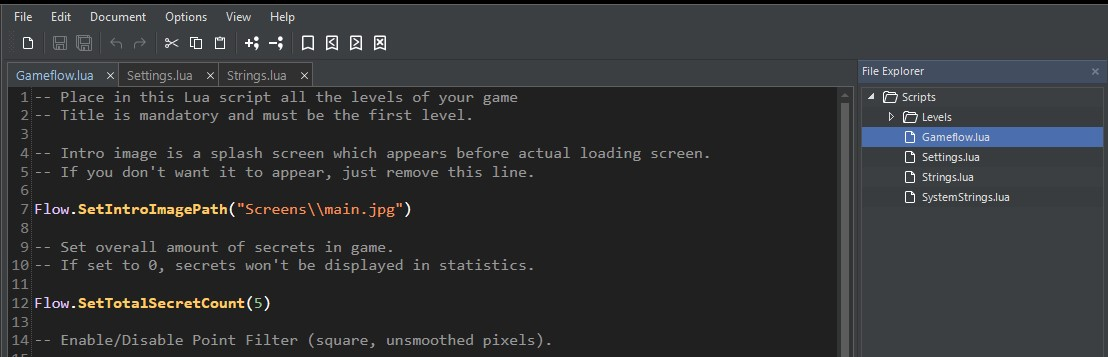
\includegraphics[width=1\textwidth]{screenshots/19.jpg}
     \caption{TombIDE Scripting Studio}
     \label{fig:TIDEScriptingStudio} 
\end{figure}

\section{Visual Studio Code \index{Visual Studio Code} \index{VSCode}}

\subsection{What is VS Code?}
\textbf{Visual Studio Code (VS Code)} is an integrated development environment developed by Microsoft for Windows, Linux, macOS and web browsers. Features include support for debugging, syntax highlighting, intelligent code completion, snippets, code refactoring, and embedded version control with Git. Users can change the theme, keyboard shortcuts and preferences, as well as install extensions that add functionality.

\par Visual Studio Code is proprietary software released under the "Microsoft Software License", but based on the MIT licensed program named "Visual Studio Code - Open Source" (also known as "Code - OSS"), also created by Microsoft and available through GitHub.

\par In the 2024 Stack Overflow Developer Survey, out of 58,121 responses, 73.6\% of respondents reported using Visual Studio Code, more than twice the percentage of respondents who reported using its nearest alternative, Visual Studio. \cite{VSCode_Wikipedia}

\subsection{Integration with TIDE}
Once installed VS Code on your PC, you can click on the \emph{Open Project in Visual Studio Code...} button on the left side of TombIDE. This action opens VS Code automatically placed on the \path{Engine \ Scripts} folder and opens the \path{Gameflow.lua} script.
\par Furthermore, if not installed already, TIDE will propose you to install the \emph{Lua language server} extension in VS Code \footnote{The \emph{Lua language server} extension provides various language features for Lua to make development easier and faster. With nearly a million installs in Visual Studio Code, it is the most popular extension for Lua language support.}.

\section{Gameflow.lua}

This script file exists initially in TE pack, and always very simple. However, it is crucial, your level won't run in the game (properly) if you do not set here the main data of the level (properly).
Gameflow.lua is is separated into three parts with the 
\begin{lstlisting}[style=lua]
--------------------------------------------------
\end{lstlisting}
 rows (which are comments, because they are start with 
\begin{lstlisting}[style=lua]
--
\end{lstlisting}
signs):
\begin{itemize}
    \item In the first (uppermost) part there are some \textbf{general settings of the game}, like eg. the maximum number of secrets. - This part is unimportant to us now (because their default values are nicely useable - or, at least, their effect is currently irrelevant), so we skip it.
    \item In the second (middle) part you can find the \textbf{level block for the title}, existing initially. Yes, as I said, technically the title is also a level - but we won't discuss it now, it is not a title tutorial. What matters is it works nicely for your project even now, so now you don't need to care about its default script values or any other part. (Though, as I said, it is not the well-known The Last Revelation title, but something much simpler.) \\ However, you need to know that not the "title" name turns a level into title, but the fact that its level block is the first (uppermost) level block in Gameflow.lua.
    \item In the third (lowest) part you can find the \textbf{level blocks for all the "real" (i.e. non-title) levels of your game}. This part is initially empty, but, when a wizard creates a level for the project, then the level block for this level will be automatically created (placed in the order of creating those levels).
\end{itemize}

So what we are interested in now is how this level block looks for \path{Test1.prj2}, which the rows and their default values are in this block.
Initial level block rows are simple commands for that level. ("Officially" I shouldn't call them commands, but something else. However, I bet you will remember them more easily, if I call them commands. In latter tutorials we will be more precise, but in a basic one like this it is enough.) - These commands are, from above to bottom (technically the command order doesn't really seem important here, though):

\begin{lstlisting}[style=lua]
Test1 = TEN.Flow.Level()
\end{lstlisting}

This command indicates that here starts a level block. The Test1 tag of the command indicates that all the commands of this block will start with this tag.

\begin{lstlisting}[style=lua]
Test1.nameKey = "Test1"
\end{lstlisting}

It tells that the name key of this level will be Test1. (Please notice that title level has no name key defined this way.)
As you can see, the command tag is the name key you set. But it is not necessary, you can change the tag manually even now, so they will be different. (Technically you can also change the name key manually - but don't forget to change it in all the places where it is already used.)

\begin{lstlisting}[style=lua]
Test1.scriptFile = "Scripts\\Levels\\Test1.lua"
\end{lstlisting}

As I told above, there should be a LUA file with the name key of the level in \path{Scripts\Levels} folder, which file is defined here. (Please notice that \path{\\} sign are used instead of \path{\} sign.)

\begin{lstlisting}[style=lua]
Test1.ambientTrack = "110"
\end{lstlisting}

As you set it previously, the initial ambience background noise for the level should be 110.wav.

\begin{lstlisting}[style=lua]
Test1.horizon1.enabled = true
\end{lstlisting}
As you set it previously, the sky above you can be visible in the outdoor areas of the level. (That is why it is "true".) Please note from \path{horizon1} that even more than one horizon are available at the same time.

\begin{lstlisting}[style=lua]
Test1.levelFile = "Data\\Test1.ten"
\end{lstlisting}
As I told above, the playable level that belongs to Test1.prj2 level map should be called Test1.ten. And, as I also told above, each TEN file will be automatically available in \path{Engine\Data} subfolder of the project main folder, including Test1.ten. These infos are defined here.

\begin{lstlisting}[style=lua]
Test1.loadScreenFile = "Screens\\loading.png"
\end{lstlisting}

This command sets the image shown when the game loads that level - this is \path{loading.jpg} now, should be placed in \path{Engine\Screens} subfolder of the project main folder.

\begin{lstlisting}[style=lua]
TEN.Flow.AddLevel(Test1)
\end{lstlisting}

This command tells that the level block for the level with Test1 tag name (not Test1 name key!) ends here, and the playable level with these block parameters is set as a part of this game.
\\
\par These default values are proper for our purposes, so we won't change them now. (But you can naturally do that later, though.)

Be awared it's possible to create Test1.prj2 level map file manually: in that case, you'll need to add this level block manually to Gameflow.lua as well. We'll see how to create a level manually later on. %Da fare

\section{Strings.lua}

The TEN script file \textbf{used to edit the texts which are seeable in the game} is called \path{Strings.lua}, existing initially in TE pack.

\par With comments, this file is also separated into parts. We are interested now only in the lower part now, which the comment names as "Level name strings".
There are some initial (and perhaps ununderstandable - but it doesn't matter now) level names are set here. But when the wizard created Test1.prj2, then a new entry was also created here, telling that the name you will see in the game for the level which has Test1 name key is Test Level 1, as you set it previously:

\begin{lstlisting}[style=lua]
Test1 = { "Test Level 1" },
\end{lstlisting}

Naturally you need to type this entry manually, if you create \path{Test1.prj2} file manually.

\section{Test1.lua}

This file has been automatically created when the wizard created Test1.prj2.
The contents of the file isn't important now, we won't use these entries now, to test this new level. (This will be the place later of the thing I've just called "additional scripting".)

\begin{lstlisting}[style=lua]
-- FILE: Levels\Test1.lua
LevelFuncs.OnLoad = function() end
LevelFuncs.OnSave = function() end
LevelFuncs.OnStart = function() end
LevelFuncs.OnLoop = function() end
LevelFuncs.OnEnd = function() end
LevelFuncs.OnUseItem = function() end
LevelFuncs.OnFreeze = function() end
\end{lstlisting}

However, the fact that this file exists by the wizard means you should create this non-existing file manually, when you create your level manually:
\begin{enumerate}
    \item There is a dropdown menu option, a toolbar button and even a shortcut key in Scripting Studio, to open a new script file. 
When you do this, a panel pops up (\ref{fig:TIDEnewfile}). Set here the file route (in Levels subfolder of Scripts folder), the file name (typing Test1) and the format (LUA), then create Test1.lua for Test Level 1. (That \path{-- FILE} comment will be automatically created now.)
    \item Type the basic contents in Test1.lua.
    \item Don't forget to refresh the script by saving in TIDE the script file you have just modified.
\end{enumerate}

\begin{figure}
    \centering
     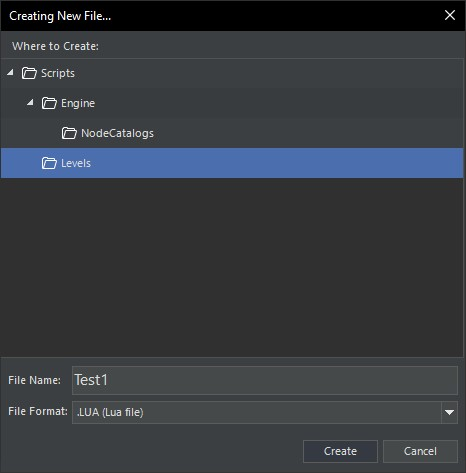
\includegraphics[width=0.75\textwidth]{screenshots/29.jpg}
     \caption{\emph{Creating new file...} popup}
     \label{fig:TIDEnewfile}
\end{figure}

\chapter{Main TE settings for the level}

The main TE settings for a level map can be checked in dropdown \path{Tools\Level Settings} menu, in Tomb Editor once opened the level.

So open Test1.prj2 in TE, and check these settings (\ref{fig:TElevelsettings}).

\begin{figure}
    \centering
     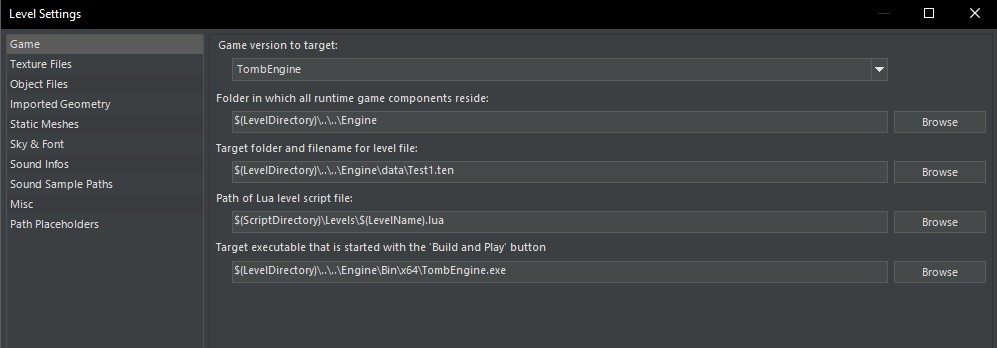
\includegraphics[width=0.75\textwidth]{screenshots/23.jpg}
     \caption{\emph{Level Settings}}
     \label{fig:TElevelsettings}
\end{figure}

If the wizard created the PRJ2 file for you, then the values here always should be the proper ones. But if you create it manually, then you need to set the proper values:
\begin{itemize}
    \item \textbf{Game version to target}: naturally you choose here TombEngine now.
    \item \textbf{Folder in which all runtime game components reside}: select Engine folder of the project main folder.
    \item \textbf{Target folder and filename for level file}: select Test1.ten in \path{Engine\Data} folder of project main folder. (I mean, Test1.ten naturally doesn't exist now if you've never built your PRJ2 level. If so, you should manually type the file name now.)
    \item \textbf{Path of Lua level script file}: select \path{Engine\Scripts\Level} folder of the project main folder.
    \item \textbf{Target executable that is started with the 'Build and Play' button}: select TombEngine.exe in \path{Engine\Bin\x64} folder of the project main folder. (Or choose the EXE in x86 folder, if your system configuration is different.)
\end{itemize}

 Don't forget to also check \emph{Misc} page here (\ref{fig:TElevelsettingsMisc}): \textbf{Full file path for the currently open level} value should be the route of this PRJ2.

 \begin{figure}
    \centering
     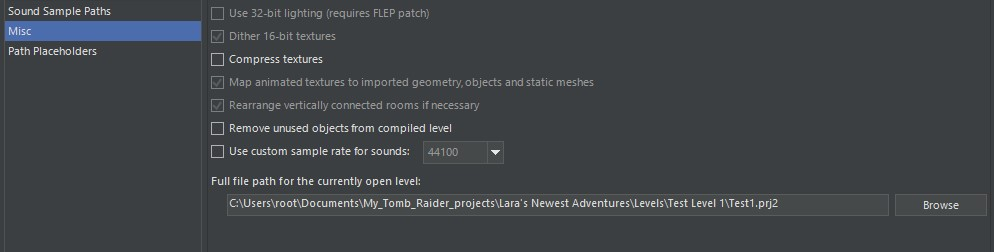
\includegraphics[width=0.75\textwidth]{screenshots/24.jpg}
     \caption{Level Settings \emph{Misc} page}
     \label{fig:TElevelsettingsMisc}
\end{figure}

\chapter{The WAD}

Open Test1.prj2 in TE now, and check these.

\section{WAD2 file}
As I said above, in TE you can select more than one WAD2 file for a TEN level. - But, for a basic tutorial like this, only one WAD2 attached is enough to us to start editing the level. That is why we are examining now only one WAD2 attached to Test1.prj2.


% Capitolo in ballo:
% \chapter{Starting a new level map}
% \section{Manually using Tomb Editor}
% Sono abbastanza scettico sul lasciare questo capitolo in questa sezione. Si può sicuramente ricordare che quanto troviamo nel livello creato dal wizard non lo troveremo se creiamo un livello a mano. Ma a mio parere è al momento inutile spiegare come creare a mano un livello ed aggiungerlo a mano. Può servire presumibilmente, al momento, per ricordare i componenti fondamentali...

% NOTA BENE: valutare in fase di revisione se parlare di Crucial Attachment. In realtà anche gli script LUA sono cruciali ed hanno la medesima importanza sostanziale del WAD, delle texture e del catalogo suoni. Secondo me tutti questi concetti hanno la stessa rilevanza ai fini di una trattazione più esaustiva possibile.

% NOTA BENE: la prima parte del tutorial di AkyV da cui è tratta questa prima parte del manuale è fondamentale per questo primo capitolo. Tuttavia ne sto cambiando la struttura ed alcune parti in prima battuta, in quanto:
% - è pensata per chi era già un builder con i vecchi editor TRLE / NGLE, si evince chiaramente leggendolo. Mentre questo manuale è pensato per un dilettante (allo sbaraglio :) )..
% - richiama più volte come creare manualmente un livello. A mio parere non è rilevante all'inizio. In prima battuta, serve capire le componenti fondamentali necessarie ad un livello per funzionare, partendo da quello che il wizard ha fatto per te ed analizzandolo. Poi entrando nel merito di WAD e quant'altro, il lettore dovrebbe arrivare a capire che si può fare tutto a manella, man mano che approfondisce i concetti (il che mi sembra piuttosto ovvio), incluso lo stesso PRJ2 con Tomb Editor.
